\paragraph{1.2.5. FastKAN/MLP Classifier (Bộ phân lớp)}
\indent\indent Tầng cuối cùng thực hiện ánh xạ từ không gian đặc trưng đồ thị sang không gian nhãn xác suất, sử dụng FastKAN hoặc MLP như minh họa tại \textbf{Hình \ref{fig:KTClassifier}}.

\begin{figure}[H]
    \centering
    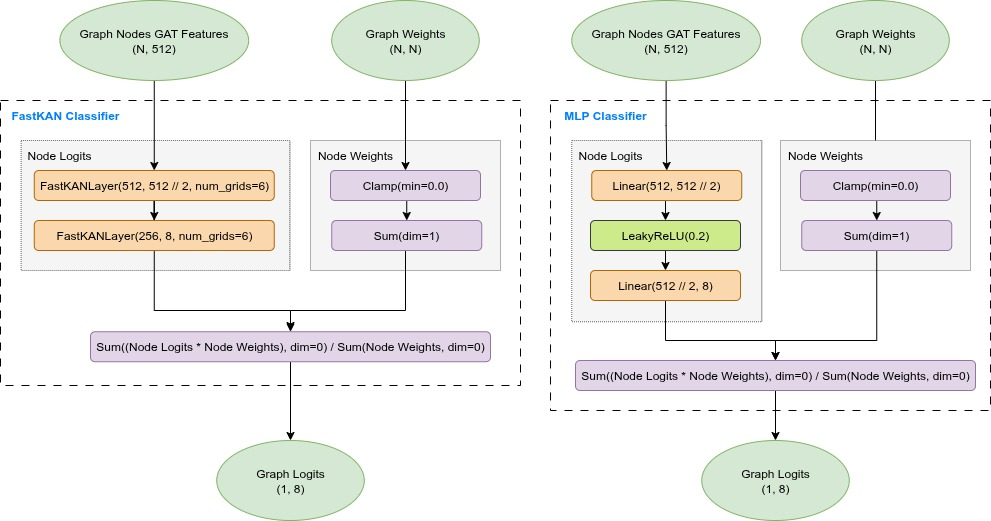
\includegraphics[width=\linewidth]{images/part-02/chap-02/sec-01/Classifier.jpg}
    \vspace{0.3cm}
    \caption{Kiến trúc bộ phân lớp bằng FastKAN và MLP}
    \label{fig:KTClassifier}
\end{figure}

Thay vì sử dụng kỹ thuật Global Mean Pooling thông thường (coi vai trò các nút là như nhau), mô hình áp dụng cơ chế Weighted Pooling (trung bình có trọng số). Kết quả dự đoán cuối cùng là trung bình có trọng số của các dự đoán từ từng nút ($logits_i$), với trọng số của mỗi nút được tính dựa trên tổng trọng số cạnh dương ($d_i = \sum_j w_{ij}$) của nút đó, với công thức cụ thể như sau:
\[
    y_{pred} = \frac{\sum_i (logits_i \cdot d_i)}{\sum_i d_i + \epsilon}
\]
\indent Trong đó $\epsilon$ là hằng số nhỏ để tránh lỗi chia cho 0. Cơ chế này phù hợp với lý thuyết về Graph Readout Operations, khẳng định rằng việc tổng hợp thông tin dựa trên cấu trúc giúp mô hình ưu tiên các nút giàu thông tin và giảm thiểu tác động của các nút ngoại lai lên kết quả dự đoán cuối cùng \cite{xu2019powerfulgraphneuralnetworks}.